\section{lla.c File Reference}
\label{lla_8c}\index{lla.c@{lla.c}}
{\tt \#include $<$stdio.h$>$}\par
{\tt \#include \char`\"{}ueaclib.h\char`\"{}}\par
{\tt \#include \char`\"{}ueac.h\char`\"{}}\par
{\tt \#include \char`\"{}lla.h\char`\"{}}\par
{\tt \#include \char`\"{}conversion.h\char`\"{}}\par
{\tt \#include \char`\"{}filter.h\char`\"{}}\par
{\tt \#include \char`\"{}global.h\char`\"{}}\par


Include dependency graph for lla.c:\begin{figure}[H]
\begin{center}
\leavevmode
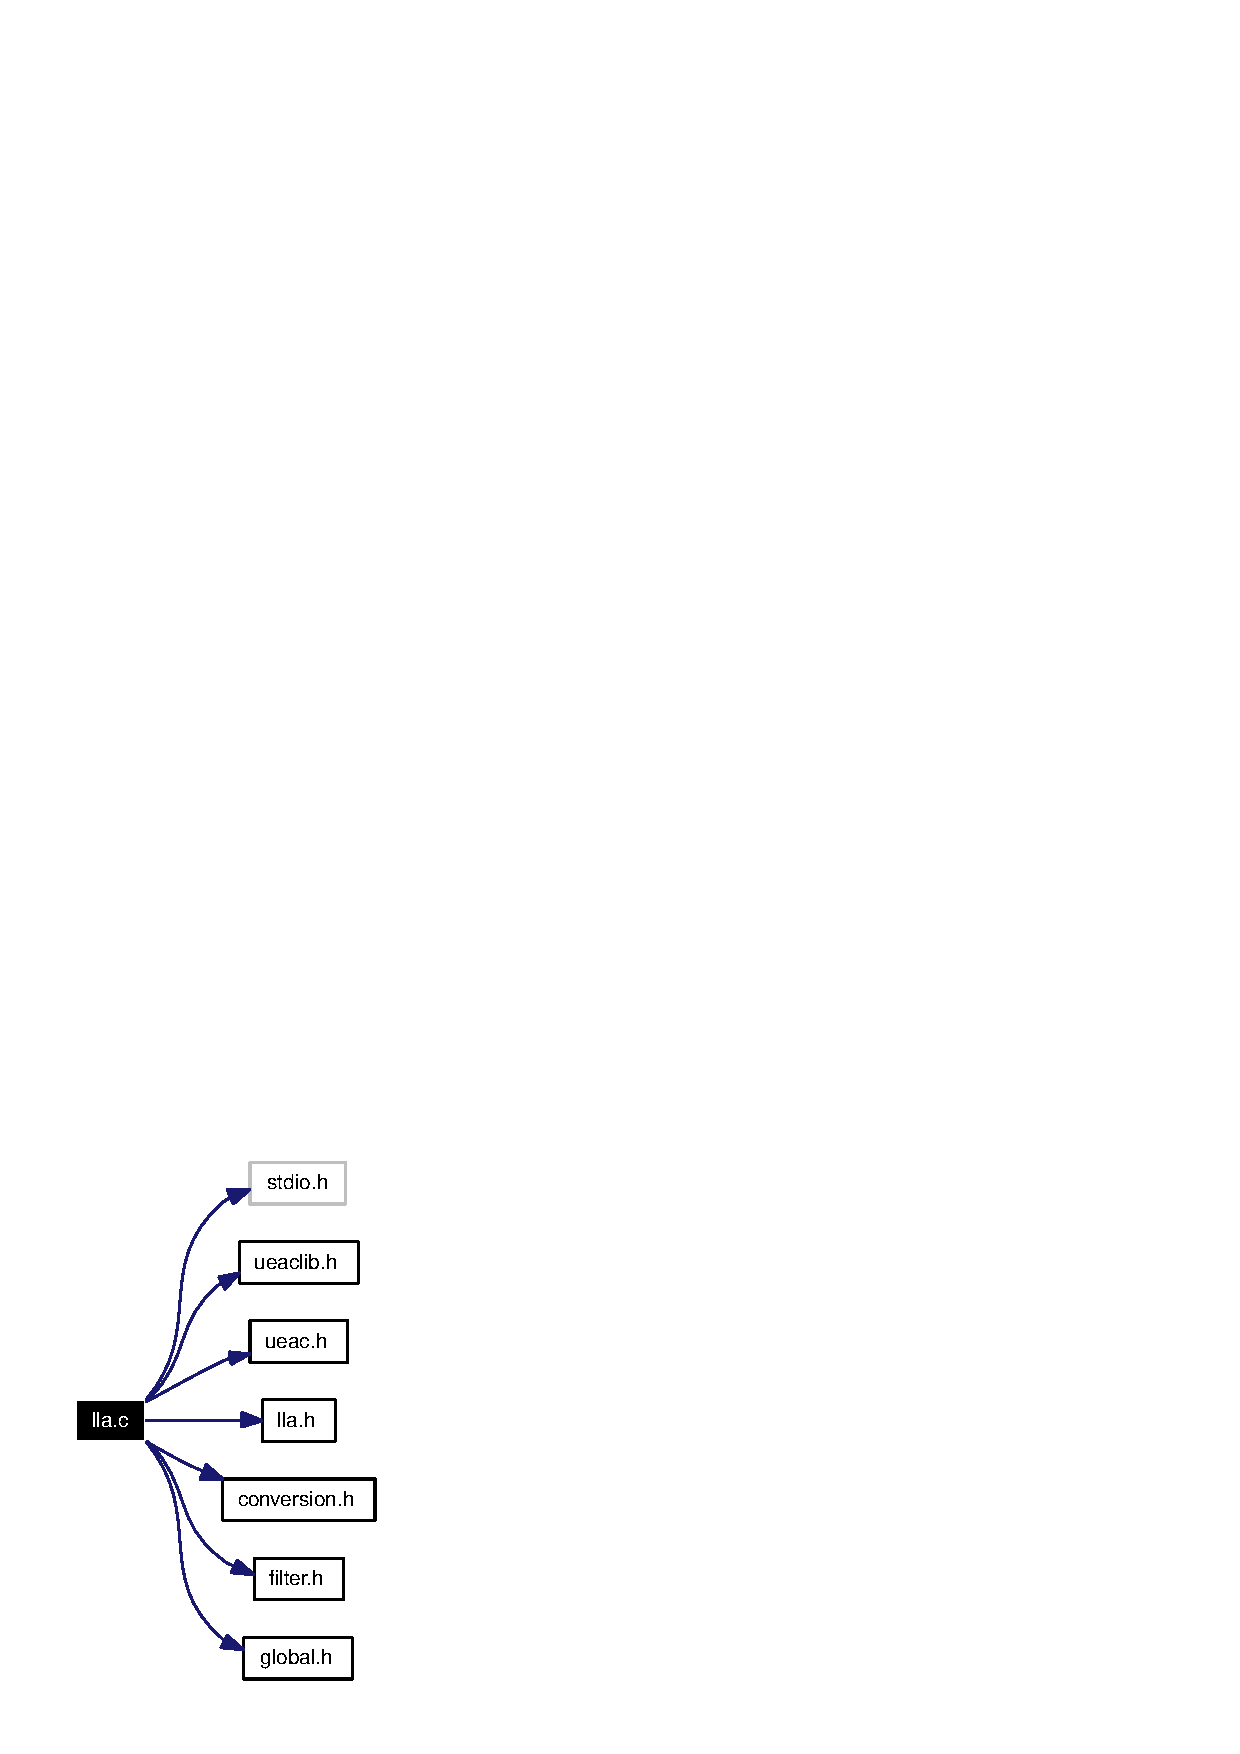
\includegraphics[width=90pt]{lla_8c__incl}
\end{center}
\end{figure}
\subsection*{Defines}
\begin{CompactItemize}
\item 
\#define {\bf INSTR}~{\bf ueac\_\-state} $\rightarrow$ instruction
\item 
\#define {\bf LLA\_\-TABLE}~{\bf ueac\_\-state} $\rightarrow$ lla\_\-table
\item 
\#define {\bf DISABLE}~0
\item 
\#define {\bf ENABLE}~1
\item 
\#define {\bf UNINITIALIZED}~0x\-FF
\end{CompactItemize}
\subsection*{Functions}
\begin{CompactItemize}
\item 
int {\bf lla\_\-report} ({\bf ueac\_\-t} $\ast${\bf ueac\_\-state}, {\bf lla\_\-data\_\-t} $\ast${\bf lla\_\-data})
\item 
int {\bf lla\_\-add} ({\bf ueac\_\-t} $\ast${\bf ueac\_\-state})
\item 
int {\bf lla\_\-disable} ({\bf ueac\_\-t} $\ast${\bf ueac\_\-state})
\item 
int {\bf lla\_\-enable} ({\bf ueac\_\-t} $\ast${\bf ueac\_\-state})
\item 
int {\bf evaluate\_\-lla} ({\bf ueac\_\-t} $\ast${\bf ueac\_\-state})
\item 
void {\bf lla\_\-print\_\-active} ({\bf ueac\_\-t} $\ast${\bf ueac\_\-state})
\end{CompactItemize}


\subsection{Define Documentation}
\index{lla.c@{lla.c}!DISABLE@{DISABLE}}
\index{DISABLE@{DISABLE}!lla.c@{lla.c}}
\subsubsection{\setlength{\rightskip}{0pt plus 5cm}\#define DISABLE~0}\label{lla_8c_a2}




Definition at line 60 of file lla.c.

Referenced by lla\_\-add(), lla\_\-disable(), and lla\_\-enable().\index{lla.c@{lla.c}!ENABLE@{ENABLE}}
\index{ENABLE@{ENABLE}!lla.c@{lla.c}}
\subsubsection{\setlength{\rightskip}{0pt plus 5cm}\#define ENABLE~1}\label{lla_8c_a3}




Definition at line 61 of file lla.c.

Referenced by evaluate\_\-lla(), lla\_\-add(), lla\_\-disable(), lla\_\-enable(), lla\_\-print\_\-active(), and lla\_\-report().\index{lla.c@{lla.c}!INSTR@{INSTR}}
\index{INSTR@{INSTR}!lla.c@{lla.c}}
\subsubsection{\setlength{\rightskip}{0pt plus 5cm}\#define INSTR~{\bf ueac\_\-state} $\rightarrow$ instruction}\label{lla_8c_a0}




Definition at line 57 of file lla.c.

Referenced by lla\_\-add(), lla\_\-disable(), lla\_\-enable(), and lla\_\-report().\index{lla.c@{lla.c}!LLA_TABLE@{LLA\_\-TABLE}}
\index{LLA_TABLE@{LLA\_\-TABLE}!lla.c@{lla.c}}
\subsubsection{\setlength{\rightskip}{0pt plus 5cm}\#define LLA\_\-TABLE~{\bf ueac\_\-state} $\rightarrow$ lla\_\-table}\label{lla_8c_a1}




Definition at line 58 of file lla.c.\index{lla.c@{lla.c}!UNINITIALIZED@{UNINITIALIZED}}
\index{UNINITIALIZED@{UNINITIALIZED}!lla.c@{lla.c}}
\subsubsection{\setlength{\rightskip}{0pt plus 5cm}\#define UNINITIALIZED~0x\-FF}\label{lla_8c_a4}




Definition at line 62 of file lla.c.

\subsection{Function Documentation}
\index{lla.c@{lla.c}!evaluate_lla@{evaluate\_\-lla}}
\index{evaluate_lla@{evaluate\_\-lla}!lla.c@{lla.c}}
\subsubsection{\setlength{\rightskip}{0pt plus 5cm}int evaluate\_\-lla ({\bf ueac\_\-t} $\ast$ {\em ueac\_\-state})}\label{lla_8c_a9}




Definition at line 134 of file lla.c.

References convert\_\-a2d(), ENABLE, I\_\-CONVERSION, ueacval::integer, LLA\_\-TABLE, pin\_\-data, and write\_\-current().

Referenced by timer\_\-a0\_\-irq().

\footnotesize\begin{verbatim}134                                      {
135   ueacval_t result;
136   static unsigned char count=0;
137   if (++count>9) {
138     count=0;
139   }
140   if (LLA_TABLE[count].enable==ENABLE) {
141 #ifndef LINUX
142     convert_a2d(I_CONVERSION,pin_data[LLA_TABLE[count].in_pin].filtered_result,&result,LLA_TABLE[count].in_pin);
143 #else 
144     convert_a2d(I_CONVERSION,0,&result,25);
145 #endif
146     LLA_TABLE[count].in_val=result.integer;      
147     if (++LLA_TABLE[count].counter>=LLA_TABLE[count].period) {
148       LLA_TABLE[count].counter=0;
149       LLA_TABLE[count].accumulator+=LLA_TABLE[count].in_val;
150       LLA_TABLE[count].in_val=(int)(LLA_TABLE[count].accumulator/LLA_TABLE[count].period);
151       if (LLA_TABLE[count].in_val>200) {
152         LLA_TABLE[count].out_val=*(LLA_TABLE[count].function_ptr+200);
153       }
154       else {
155         LLA_TABLE[count].out_val=*(LLA_TABLE[count].function_ptr+LLA_TABLE[count].in_val);
156       }
157       if (LLA_TABLE[count].out_pin!=0xFF) {
158 #ifndef LINUX
159         write_current(LLA_TABLE[count].out_pin,LLA_TABLE[count].out_val);
160 #endif
161       }
162       LLA_TABLE[count].accumulator=0;
163     }
164     else {
165       LLA_TABLE[count].accumulator+=LLA_TABLE[count].in_val;
166     }
167   }
168   return (0);
169 }
\end{verbatim}\normalsize 




Here is the call graph for this function:\begin{figure}[H]
\begin{center}
\leavevmode
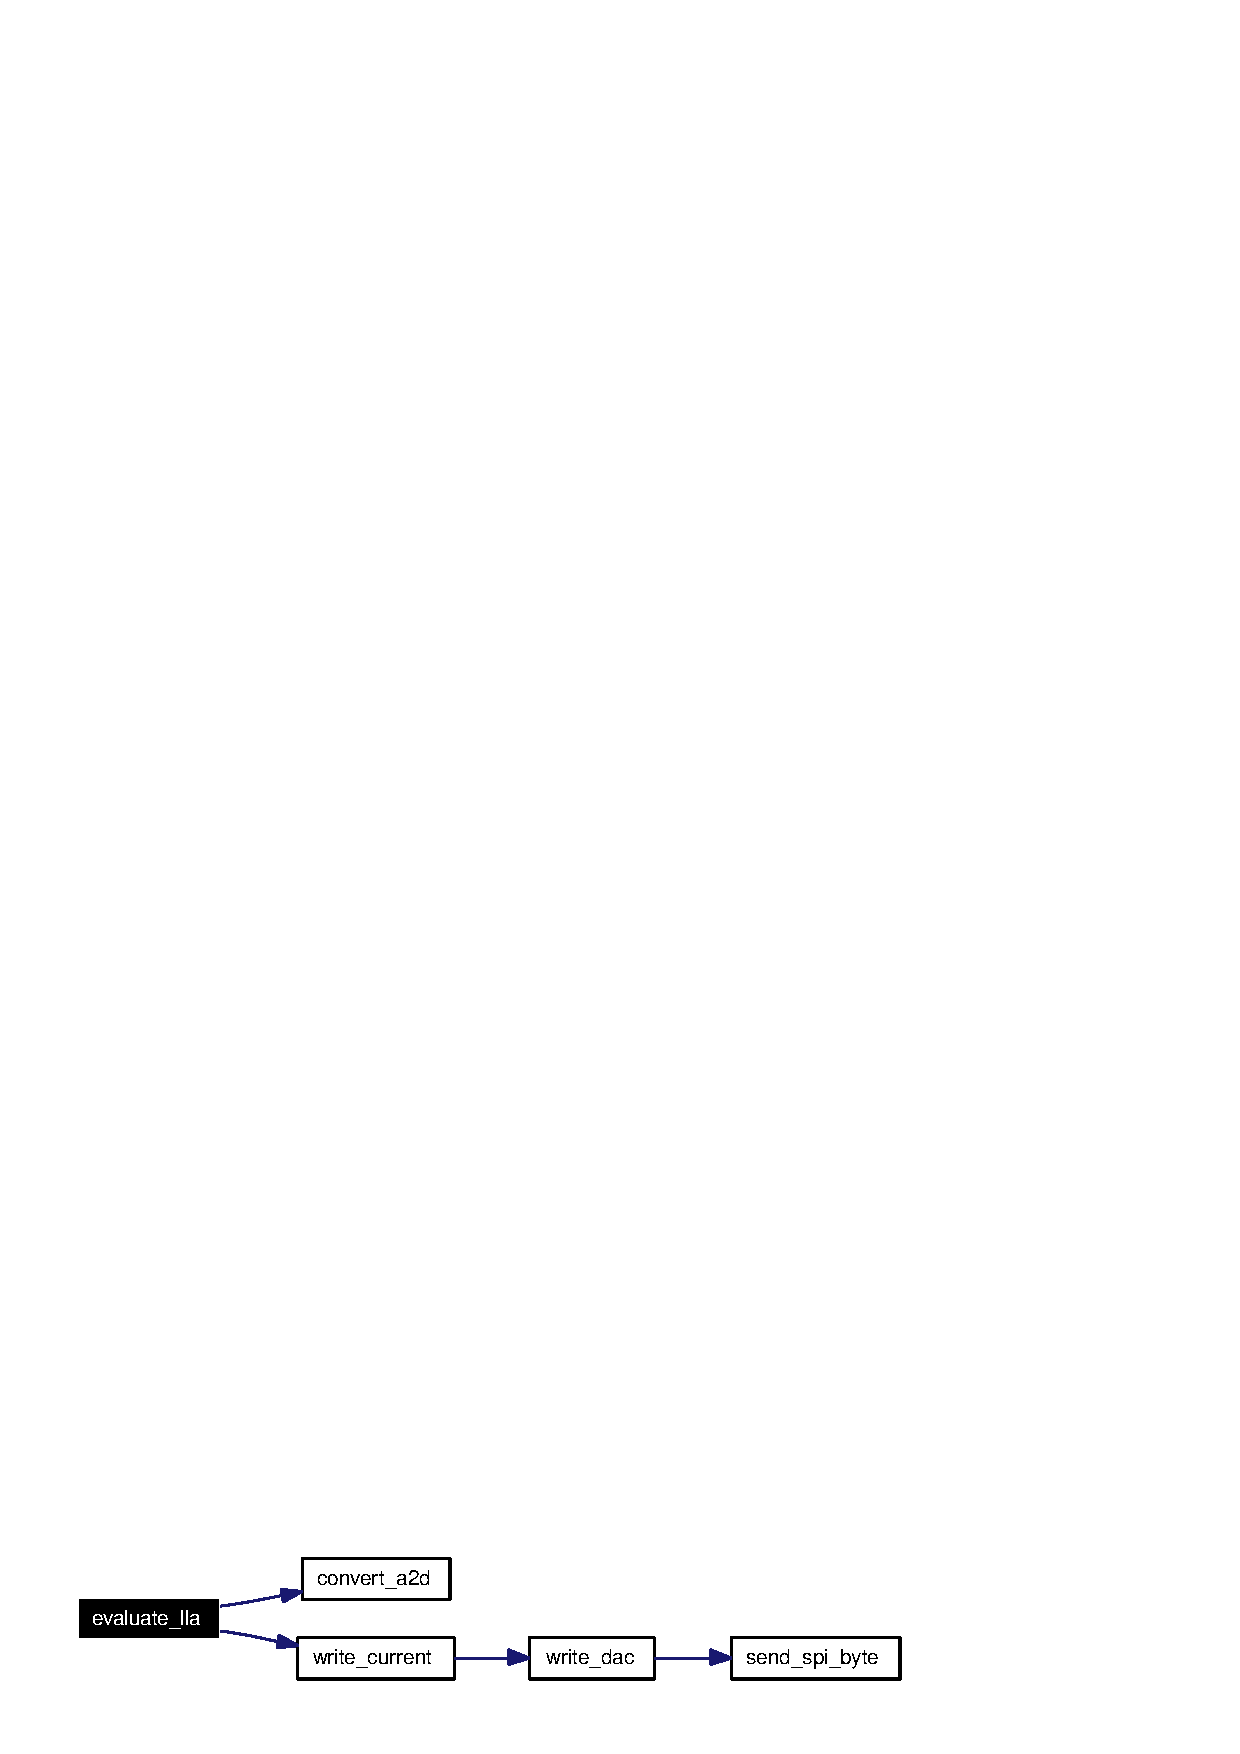
\includegraphics[width=216pt]{lla_8c_a9_cgraph}
\end{center}
\end{figure}
\index{lla.c@{lla.c}!lla_add@{lla\_\-add}}
\index{lla_add@{lla\_\-add}!lla.c@{lla.c}}
\subsubsection{\setlength{\rightskip}{0pt plus 5cm}int lla\_\-add ({\bf ueac\_\-t} $\ast$ {\em ueac\_\-state})}\label{lla_8c_a6}




Definition at line 76 of file lla.c.

References DISABLE, ENABLE, INSTR, lla\_\-function\_\-index, ueac::lla\_\-input, LLA\_\-TABLE, and write\_\-lla().

Referenced by ueac\_\-execute\_\-instruction().

\footnotesize\begin{verbatim}76                                  {
77   int index;
78   index=INSTR.lla_descriptor-1;
79   LLA_TABLE[index].enable=DISABLE;
80   LLA_TABLE[index].in_pin=(INSTR.pin_y-1)*5+(INSTR.pin_x-1);
81   if ((INSTR.pin_x_alt==0)||(INSTR.pin_y_alt==0)) {
82     LLA_TABLE[index].out_pin=0xFF;
83   }
84   else {
85     LLA_TABLE[index].out_pin=(INSTR.pin_y_alt-1)*5+(INSTR.pin_x_alt-1);
86   }
87   LLA_TABLE[index].function_ptr=(int *)lla_function_index[INSTR.lla_function-1];
88   LLA_TABLE[index].period=INSTR.lla_period;
89   LLA_TABLE[index].accumulator=0;
90   ueac_state->lla_input|=(unsigned long)(0x00000001<<LLA_TABLE[index].in_pin);
91 #ifndef LINUX 
92   write_lla(LLA_TABLE[index].in_pin,1);
93 #endif 
94   LLA_TABLE[index].in_val=0;
95   LLA_TABLE[index].out_val=0;
96   LLA_TABLE[index].enable=ENABLE;
97   return 0;
98 }
\end{verbatim}\normalsize 




Here is the call graph for this function:\begin{figure}[H]
\begin{center}
\leavevmode
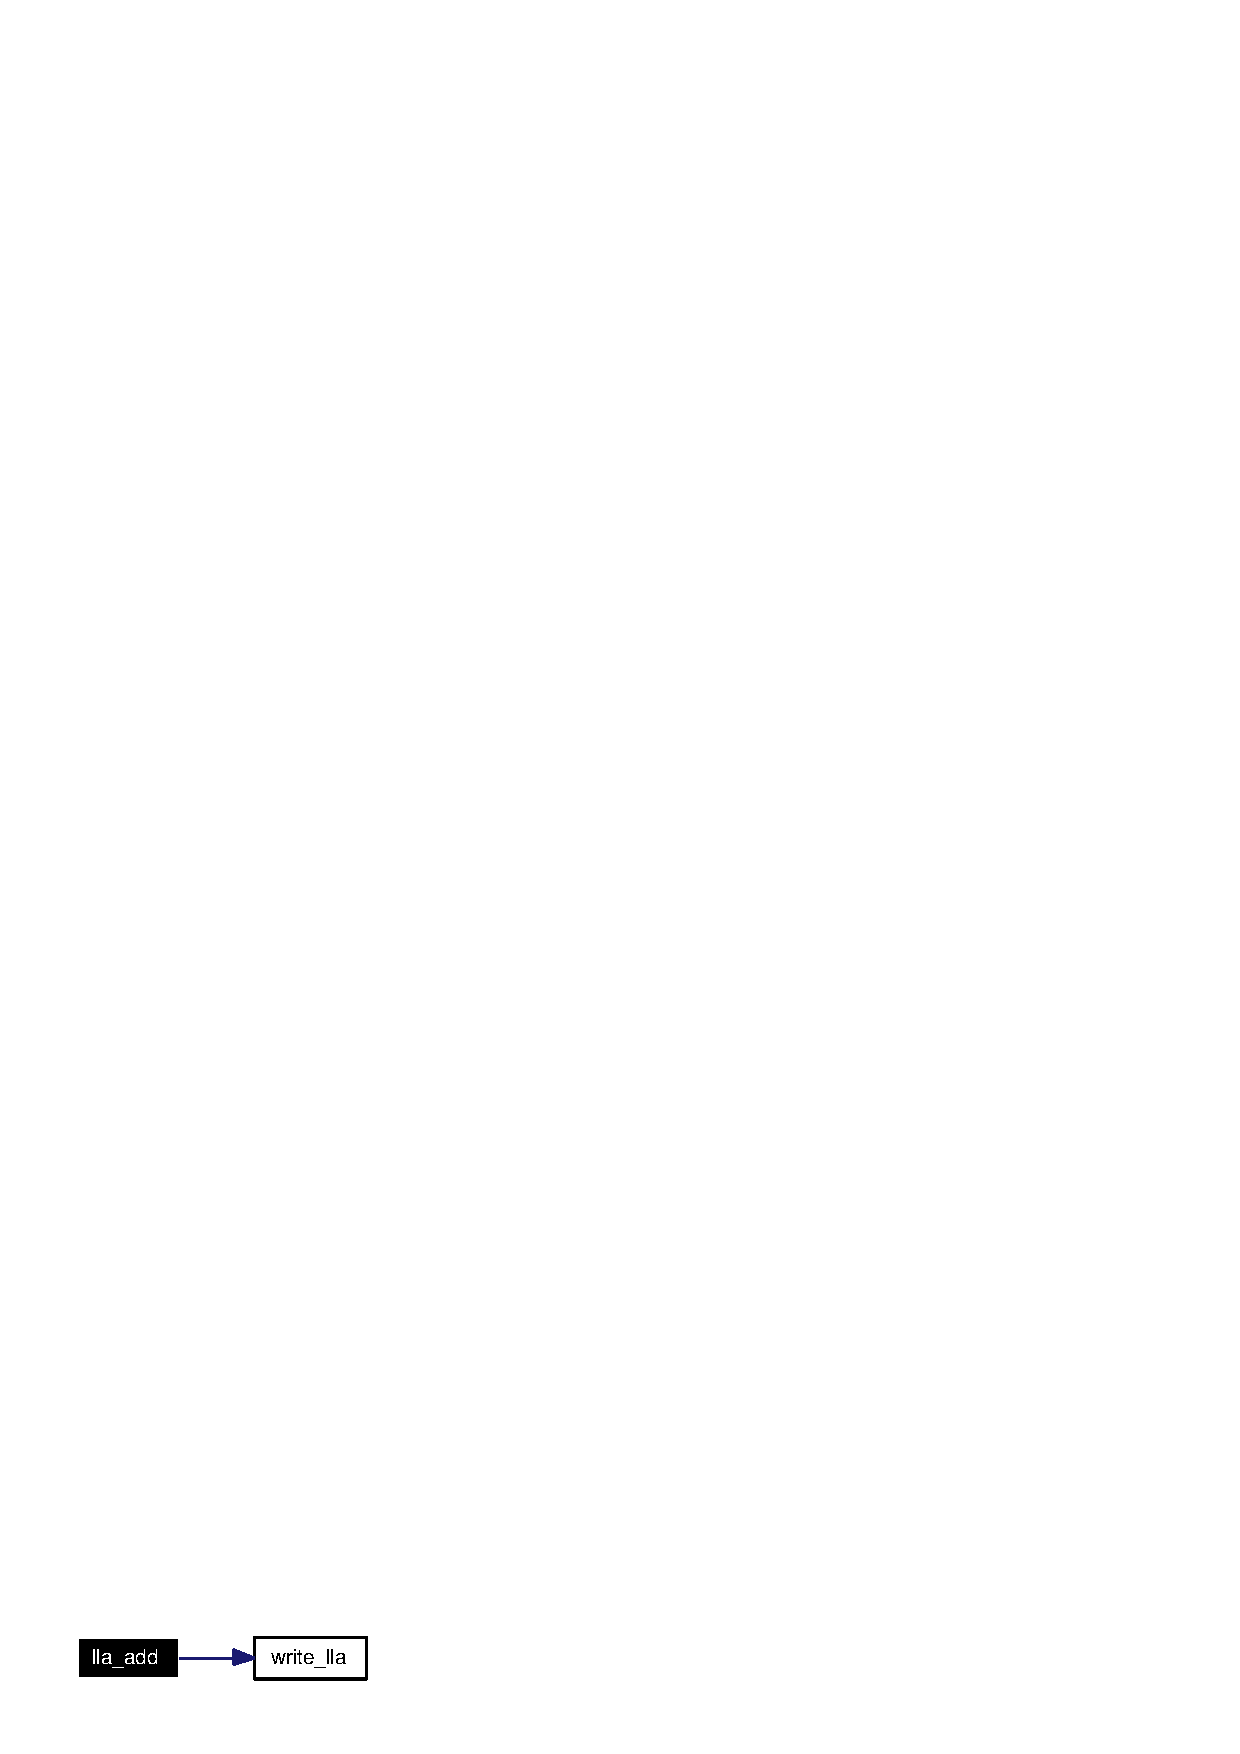
\includegraphics[width=88pt]{lla_8c_a6_cgraph}
\end{center}
\end{figure}
\index{lla.c@{lla.c}!lla_disable@{lla\_\-disable}}
\index{lla_disable@{lla\_\-disable}!lla.c@{lla.c}}
\subsubsection{\setlength{\rightskip}{0pt plus 5cm}int lla\_\-disable ({\bf ueac\_\-t} $\ast$ {\em ueac\_\-state})}\label{lla_8c_a7}




Definition at line 100 of file lla.c.

References DISABLE, ENABLE, INSTR, ueac::lla\_\-input, LLA\_\-TABLE, write\_\-current(), and write\_\-lla().

Referenced by ueac\_\-execute\_\-instruction().

\footnotesize\begin{verbatim}100                                      {
101   int index;
102   int ret_val=-1;
103   index=INSTR.lla_descriptor-1;
104   if (LLA_TABLE[index].enable==ENABLE) {
105     ueac_state->lla_input&=~((unsigned long)(0x00000001<<LLA_TABLE[index].in_pin));
106     LLA_TABLE[index].enable=DISABLE;
107 #ifndef LINUX    
108     write_lla(LLA_TABLE[index].in_pin,0);
109     write_current(LLA_TABLE[index].out_pin,0);
110 #endif 
111     ret_val=0;
112   }
113   return(ret_val);
114 }
\end{verbatim}\normalsize 




Here is the call graph for this function:\begin{figure}[H]
\begin{center}
\leavevmode
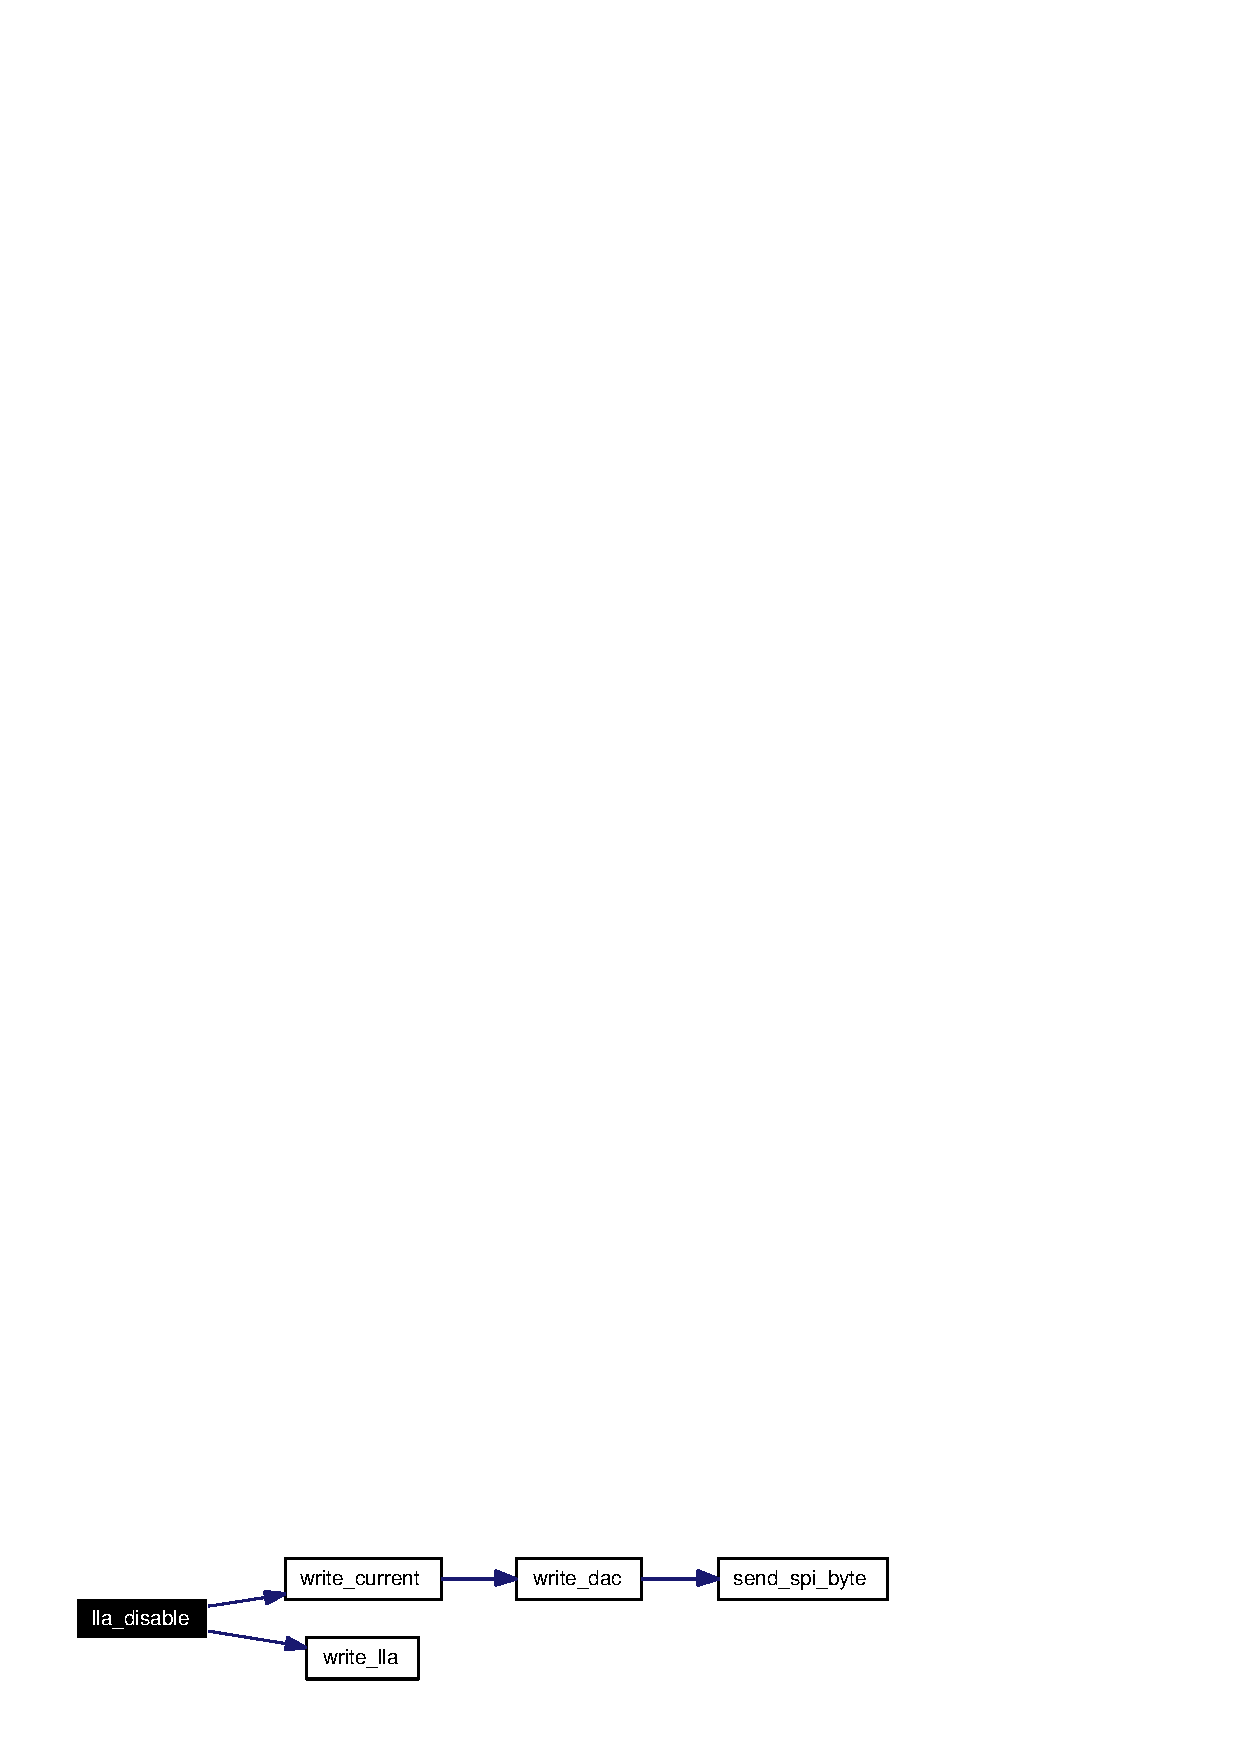
\includegraphics[width=213pt]{lla_8c_a7_cgraph}
\end{center}
\end{figure}
\index{lla.c@{lla.c}!lla_enable@{lla\_\-enable}}
\index{lla_enable@{lla\_\-enable}!lla.c@{lla.c}}
\subsubsection{\setlength{\rightskip}{0pt plus 5cm}int lla\_\-enable ({\bf ueac\_\-t} $\ast$ {\em ueac\_\-state})}\label{lla_8c_a8}




Definition at line 116 of file lla.c.

References DISABLE, ENABLE, INSTR, ueac::lla\_\-input, LLA\_\-TABLE, write\_\-current(), and write\_\-lla().

Referenced by ueac\_\-execute\_\-instruction().

\footnotesize\begin{verbatim}116                                     {
117   int index;
118   int ret_val=-1;
119   index=INSTR.lla_descriptor-1;
120   if (LLA_TABLE[index].enable==DISABLE) {
121     ueac_state->lla_input|=(unsigned long)(0x00000001<<LLA_TABLE[index].in_pin);
122 #ifndef LINUX
123     write_lla(LLA_TABLE[index].in_pin,1);
124     write_current(LLA_TABLE[index].out_pin,0);
125 #endif 
126     LLA_TABLE[index].in_val=0;
127     LLA_TABLE[index].out_val=0;
128     LLA_TABLE[index].enable=ENABLE;
129     ret_val=0;
130   }
131   return(ret_val);
132 }
\end{verbatim}\normalsize 




Here is the call graph for this function:\begin{figure}[H]
\begin{center}
\leavevmode
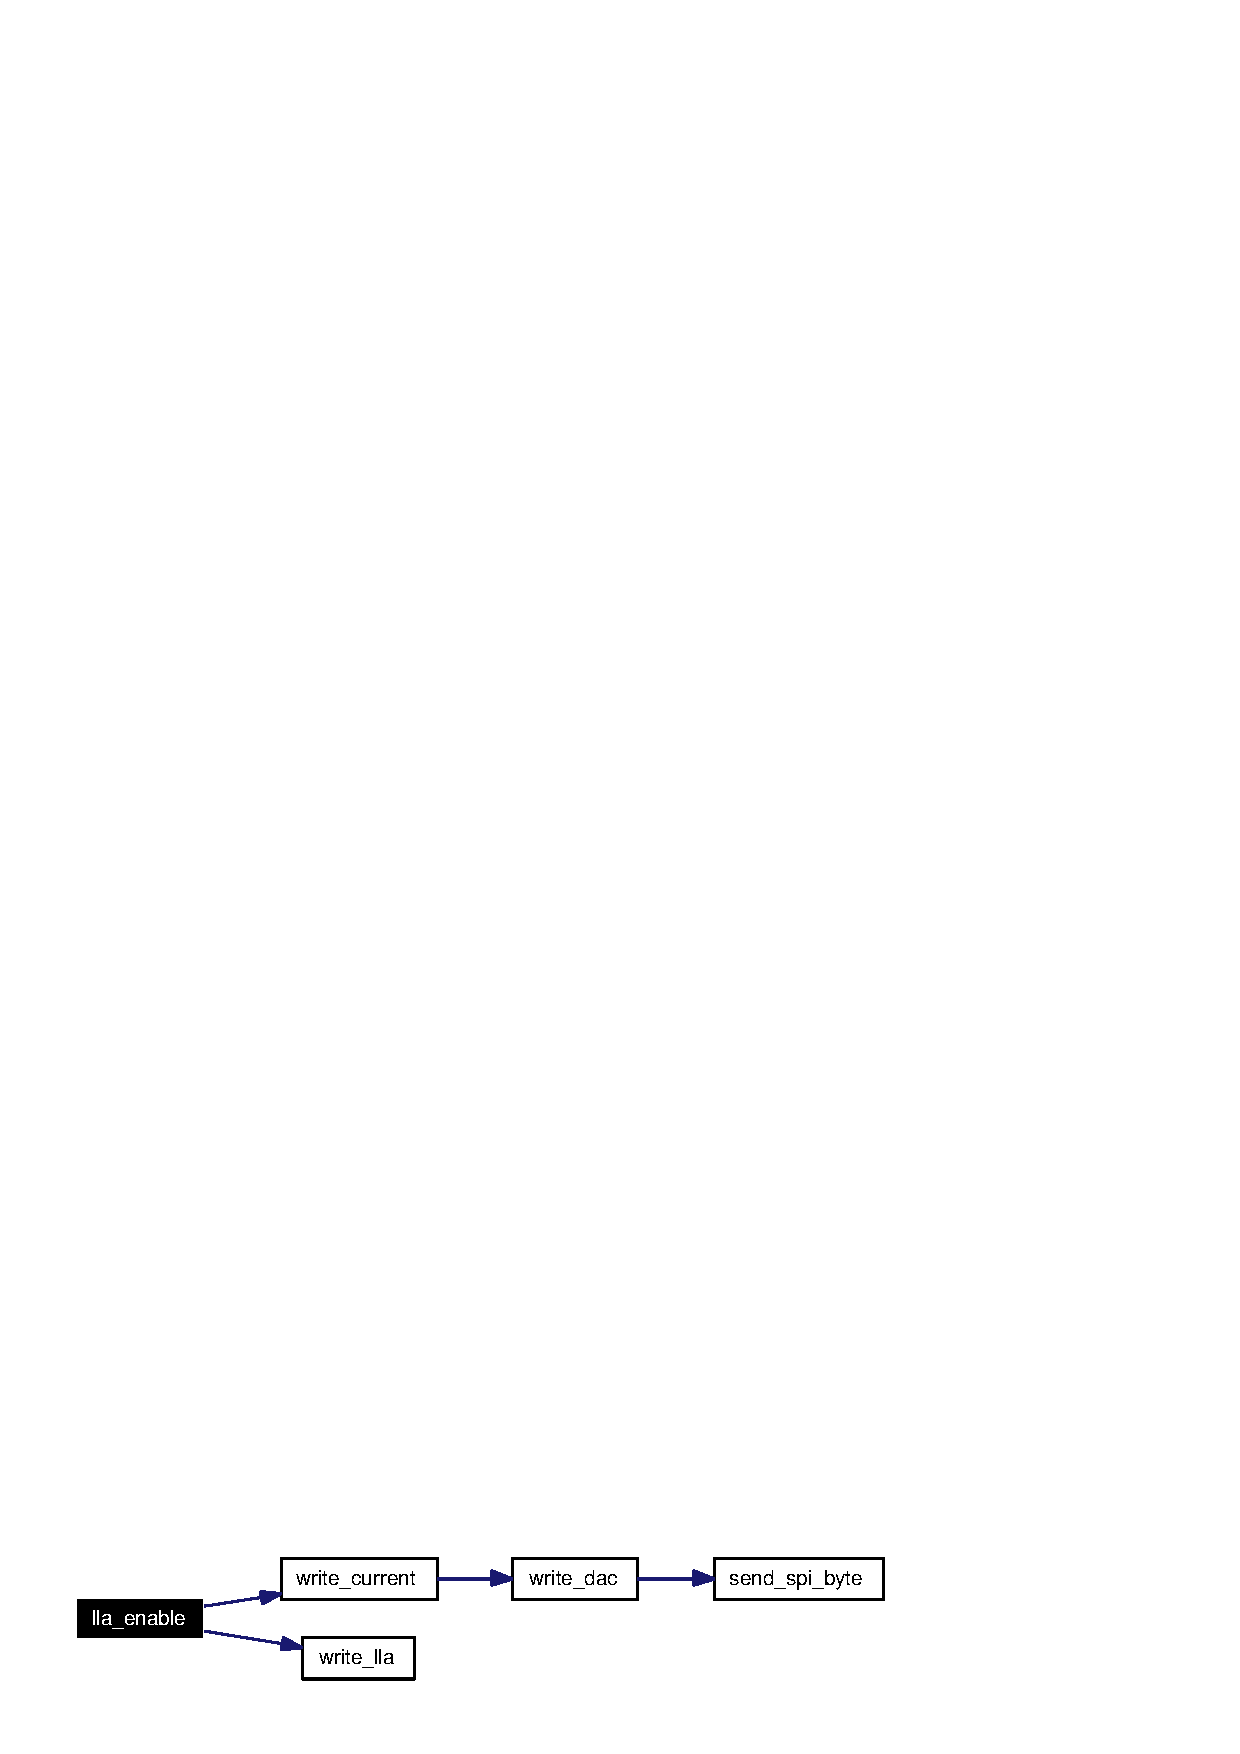
\includegraphics[width=212pt]{lla_8c_a8_cgraph}
\end{center}
\end{figure}
\index{lla.c@{lla.c}!lla_print_active@{lla\_\-print\_\-active}}
\index{lla_print_active@{lla\_\-print\_\-active}!lla.c@{lla.c}}
\subsubsection{\setlength{\rightskip}{0pt plus 5cm}void lla\_\-print\_\-active ({\bf ueac\_\-t} $\ast$ {\em ueac\_\-state})}\label{lla_8c_a10}




Definition at line 171 of file lla.c.

References ENABLE, ueac::lla\_\-input, and LLA\_\-TABLE.

\footnotesize\begin{verbatim}171                                            {
172   int i;
173   printf ("lla_input var=0x%08lx\n",ueac_state->lla_input);
174   for (i=0;i<10;i++) {
175 #ifdef LINUX
176     printf("\nLLA %d\n",i+1);
177     if (LLA_TABLE[i].enable==ENABLE) {
178       printf("enable state=ENABLED\n");
179       printf("input pin = %d\n",LLA_TABLE[i].in_pin);
180       printf("output pin = %d\n",LLA_TABLE[i].out_pin);
181       printf("first data val = %d\n",*(LLA_TABLE[i].function_ptr+100));
182       printf("period = %d\n",LLA_TABLE[i].period);
183       printf("in_val = %d\n",LLA_TABLE[i].in_val);
184       printf("out_val = %d\n",LLA_TABLE[i].out_val);
185       printf("accumulator = %ld\n",LLA_TABLE[i].accumulator);
186     }
187     else {
188       printf("enable state=DISABLED\n");
189     }
190 #else 
191     printf("\nLLA %d\n\r",i+1);
192     if (LLA_TABLE[i].enable==ENABLE) {
193       printf("enable state=ENABLED\n\r");
194       printf("input pin = %d\n\r",LLA_TABLE[i].in_pin);
195       printf("output pin = %d\n\r",LLA_TABLE[i].out_pin);
196       printf("first data val = %d\n\r",*(LLA_TABLE[i].function_ptr+100));
197       printf("period = %d\n\r",LLA_TABLE[i].period);
198       printf("in_val = %d\n\r",LLA_TABLE[i].in_val);
199       printf("out_val = %d\n\r",LLA_TABLE[i].out_val);
200       printf("accumulator = %ld\n\r",LLA_TABLE[i].accumulator);
201     }
202     else {
203       printf("enable state=DISABLED\n");
204     }
205 #endif
206 
207   }
208 }
\end{verbatim}\normalsize 


\index{lla.c@{lla.c}!lla_report@{lla\_\-report}}
\index{lla_report@{lla\_\-report}!lla.c@{lla.c}}
\subsubsection{\setlength{\rightskip}{0pt plus 5cm}int lla\_\-report ({\bf ueac\_\-t} $\ast$ {\em ueac\_\-state}, {\bf lla\_\-data\_\-t} $\ast$ {\em lla\_\-data})}\label{lla_8c_a5}




Definition at line 64 of file lla.c.

References ENABLE, lla\_\-data::input, INSTR, LLA\_\-TABLE, and lla\_\-data::output.

Referenced by ueac\_\-execute\_\-instruction().

\footnotesize\begin{verbatim}64                                                          {
65   int index;
66   int ret_val=-1;
67   index=INSTR.lla_descriptor-1;
68   if (LLA_TABLE[index].enable==ENABLE) {
69     lla_data->input=LLA_TABLE[index].in_val;
70     lla_data->output=LLA_TABLE[index].out_val;
71     ret_val=0;
72   }
73   return ret_val;
74 }
\end{verbatim}\normalsize 


